\documentclass{article}
\usepackage[polish]{babel}
\usepackage[T1]{fontenc}
\usepackage{lmodern}
\usepackage[utf8]{inputenc}
\usepackage{graphicx}
\usepackage{bookmark}
\usepackage{float}
\usepackage{hyperref}
\usepackage[bottom=1.5cm, right=2.5cm, left=2.5cm, top=1.5cm]{geometry}
\graphicspath{{../pliki}}



\title{%
  Cyberbezpieczeństwo - laboratoria 13 \\
  \large Wykorzystanie podatności - eskalacja uprawnień}
\author{Patryk Łuszczek 272707}
\date{\today}
\begin{document}
\maketitle
\newpage
\textbf{Wszystkie zadania zostały przedstawione podczas zajęć}




\section*{Co to są nagłówki X-Content-Type-Options i X-Frame-Options podczas korzystania
  z wyszukiwania internetowego i jak mogą chronić Twoją witrynę? Jakie są typowe
  zastosowania ataków SQL Injection (jakie akcje może wykonać osoba atakująca)?}
Nagłówki X-Content-Type-Options i X-Frame-Options to mechanizmy zabezpieczające witryny przed atakami.

\begin{itemize}
    \item X-Content-Type-Options chroni przed atakami MIME-sniffing, uniemożliwiając przeglądarce automatyczne określanie typu pliku. Ustawienie wartości "nosniff" zapobiega interpretowaniu nieodpowiednich typów plików, co zwiększa bezpieczeństwo.
    \item X-Frame-Options zabezpiecza przed clickjackingiem, czyli ukrywaniem elementów strony w ramkach. Opcje: SAMEORIGIN (ramki dozwolone tylko z tej samej domeny) oraz DENY (całkowity zakaz osadzania w ramkach).
\end{itemize}

SQL Injection to technika ataku polegająca na wstrzyknięciu kodu SQL do pól wejściowych. Może prowadzić do:

\begin{itemize}
    \item Nieautoryzowanego logowania (np. jako administrator).
    \item Kradzieży lub modyfikacji danych.
    \item Usunięcia tabel bazy danych.
    \item Wykonania złośliwego kodu na serwerze, co może skutkować jego przejęciem.
\end{itemize}

\section*{Dlaczego ważne jest, aby zachować regułę sprawdzania poprawności danych za-
  równo po stronie klienta, jak i serwera?}
Sprawdzanie poprawności danych zarówno po stronie klienta, jak i serwera jest kluczowe dla bezpieczeństwa aplikacji.

\begin{itemize}
    \item Walidacja po stronie klienta zapobiega wprowadzaniu błędnych danych, zmniejsza obciążenie serwera i ogranicza ryzyko ataków, takich jak XSS. Jednak można ją łatwo ominąć, np. wysyłając żądania HTTP bezpośrednio na serwer.
    \item Walidacja po stronie serwera zapewnia, że przetwarzane są tylko poprawne dane, chroniąc m.in. przed SQL Injection i innymi atakami.
\end{itemize}

Obie metody razem zwiększają bezpieczeństwo, minimalizując ryzyko obejścia zabezpieczeń.

\section*{Jak ograniczyć dostęp do zasobów, do których użytkownik nie ma uprawnień?}
Aby ograniczyć dostęp do nieuprawnionych zasobów, należy stosować uwierzytelnianie i autoryzację, przypisując użytkownikom odpowiednie uprawnienia. Każda akcja powinna być sprawdzana pod kątem dostępu, aby utrudnić obejście zabezpieczeń.
\section*{Seciurity Misconfiguration}
Wyniki skanowania:
\begin{figure}[H]
    \centering
    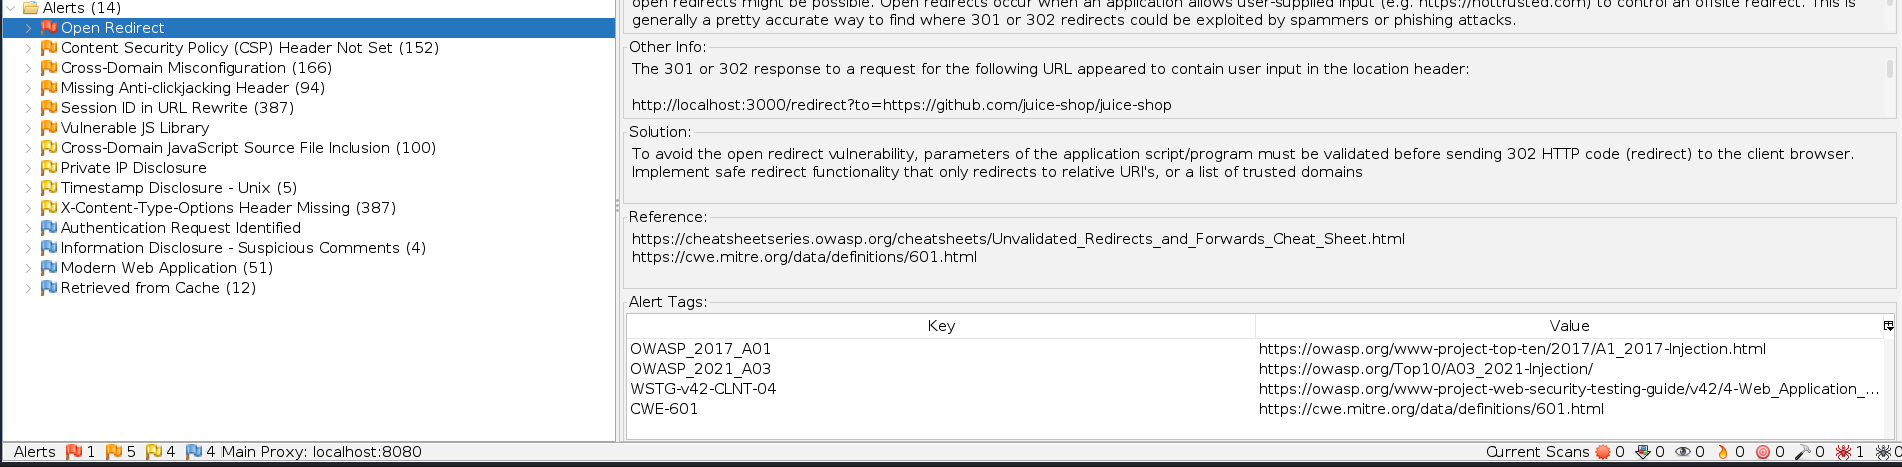
\includegraphics[width=0.8\textwidth]{open_redirect.png}
    \caption{Znalezione podatności}
\end{figure}

Odnaleziono (flagi):
\begin{itemize}
    \item Czerwonych: 1
          \begin{itemize}
              \item Open Redirect -
          \end{itemize}
    \item Bursztynowych: 5
          \begin{itemize}
              \item Vulnerable JS Library - znaleziono bibliotekę javascript ze znanymi lukami bezpieczenstwa (JQuery 2.2.4 CVE-2020-11023
                    CVE-2020-11022
                    CVE-2015-9251
                    CVE-2019-11358)
                    \begin{figure}[H]
                        \centering
                        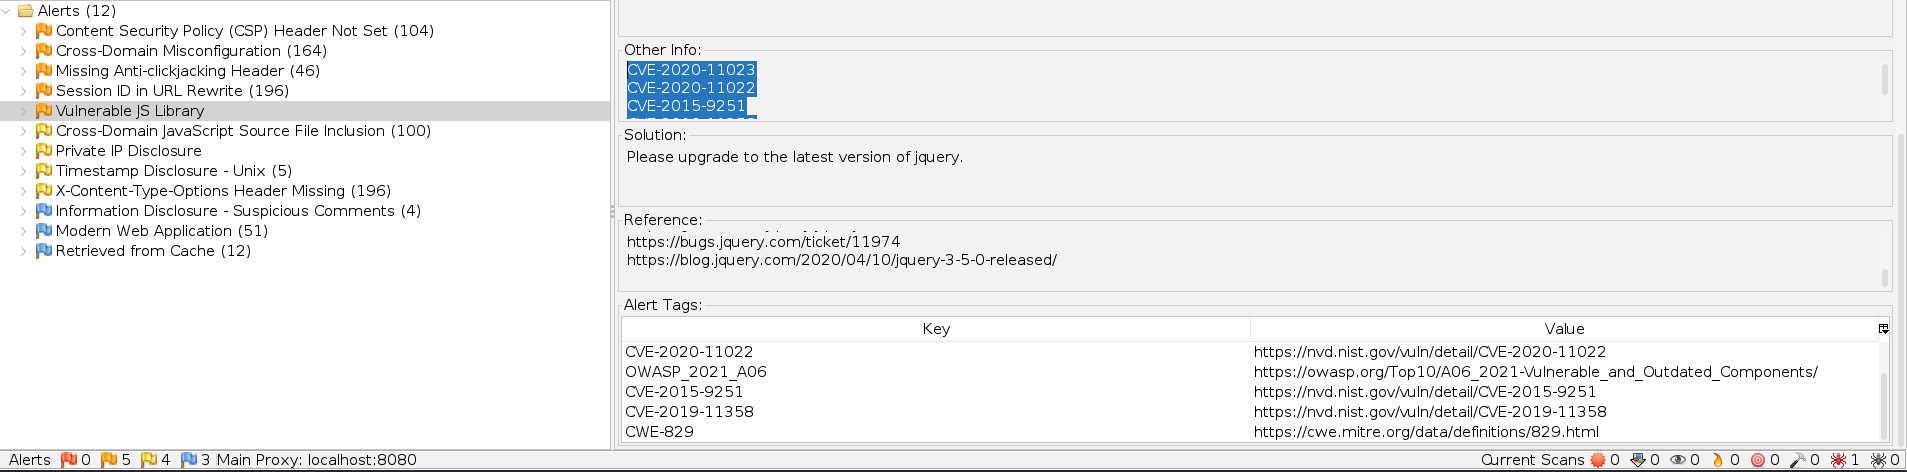
\includegraphics[width=0.8\textwidth]{jquery.png}
                    \end{figure}
          \end{itemize}
    \item Żółty: 4
          \begin{itemize}
              \item Cross-Domain JS Source File Inclusion - skrypty pochodzące z domen trzecich, które mogą być potencjalnie niebezpieczne
          \end{itemize}
    \item Niebieskie: 4
          \begin{itemize}
              \item Retrieved From Cache - dane załądowane na stronie zostały załadowane z cache, jeśli jest to wrażliwa dana, może zostać zostać ujawniona nieautoryzowanym osobom
          \end{itemize}
\end{itemize}

Znalezione katalogi:
\begin{itemize}
    \item /ftp/ - możliwość przeglądania plików
          \begin{figure}[H]
              \centering
              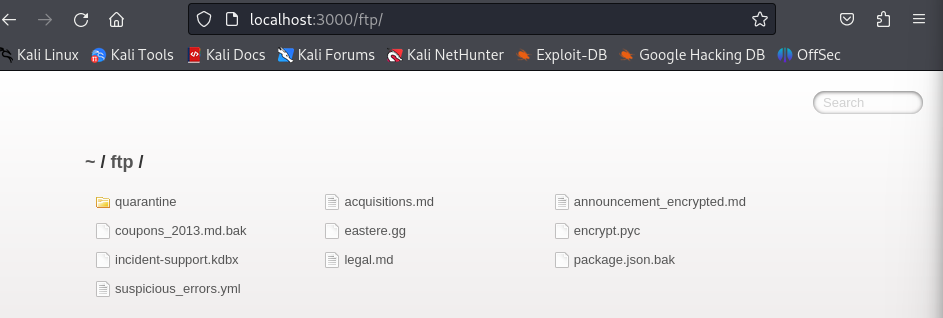
\includegraphics[width=0.8\textwidth]{katalog_ftp.png}
          \end{figure}
    \item /assets/public/images/uploads - ładuje się ale nic nie wyświetla, trzeba wpisać sćieżkę pliku
\end{itemize}

Znalezione informacje o cookies:
\begin{itemize}
    \item Burszytnowa flaga - Seesion ID in URL Rewrite - zaleca się przechowywanie session id w cookies
\end{itemize}

\section*{Improper Input Validation}
Utworzono uzytkownika z parametrami:
\texttt{"email":"a@a.a","password":"abcabc","passwordRepeat":"abcabc","question":"Mother's birth date? (MM/DD/YY)","securityAnswer":"01.01.01}
Następnie manualnie zmieniono dane w requeście, dodając pole "role":"admin" i ponownie przesłano requesta. Udało się zmienić rolę użytkownika na admina.
\begin{figure}[H]
    \centering
    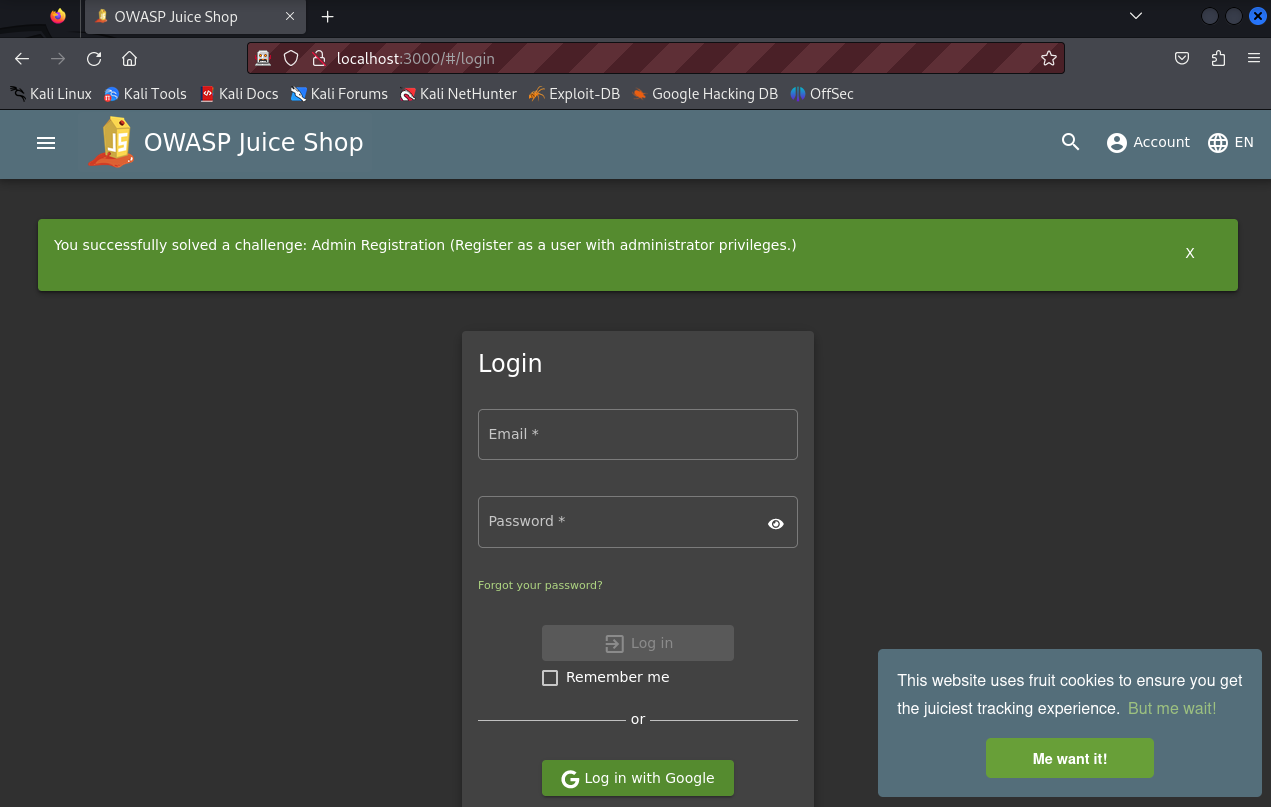
\includegraphics[width=0.8\textwidth]{admin_success.png}
    \caption{Zmiana roli użytkownika}
\end{figure}

\section*{Broken Authentication}
Utworzono użytkonika z odpowiedzią na pytanie zabezpieczające: "10.10.1980".
Użyto narzędzia do odzyskiwania hasła, w któym trzeba było wprowadzi  odpowiedź na pytanie zabezpieczające. Wprowadzonno niepoprawne dane a następnie został użyty Fuzzer do odgadnięcia odpowiedzi na pytanie zabezpieczające za pomocą brute-force.
Fuzzer poprawnie odgadł odpowiedź, a hasło zostało zresetowane.
\begin{figure}[H]
    \centering
    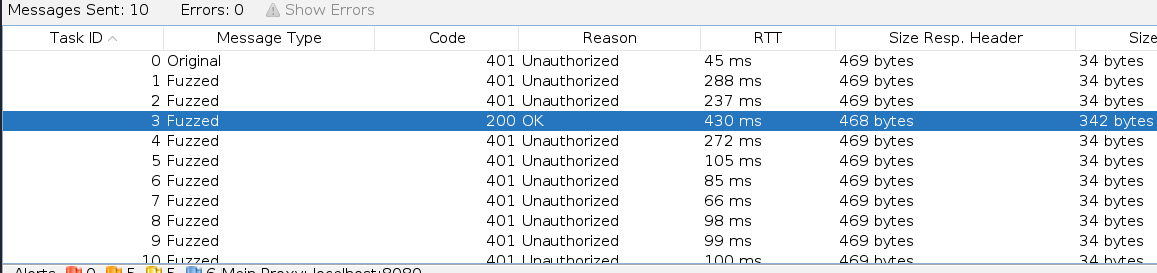
\includegraphics[width=0.8\textwidth]{fuzzer.png}
\end{figure}

\section*{Broken Access Control}
Po wejściu do koszyka zmieniono request get aby przechwycił dane o koszyku innego użytkonika. Rządanie zakończyło się sukcesem i udało się uzyskać informacje o koszyku innego użytkownika.
\begin{figure}[H]
    \centering
    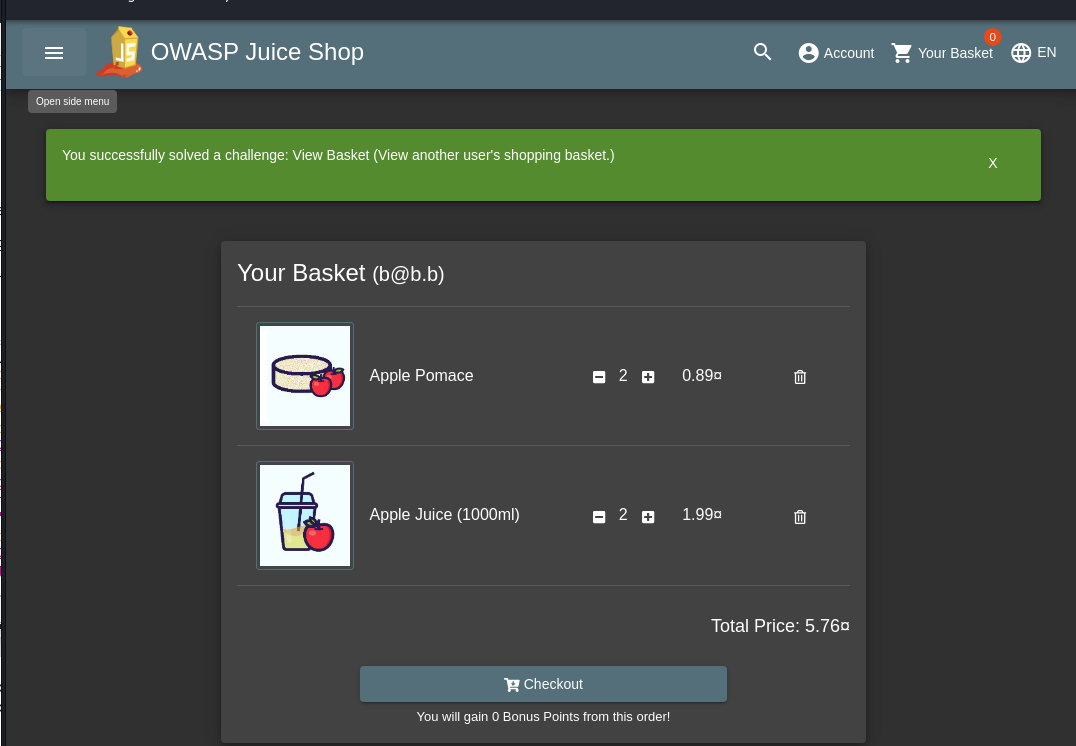
\includegraphics[width=0.8\textwidth]{basket.png}
\end{figure}

\end{document}